\documentclass[12pt,letterpaper]{article}
\usepackage{graphicx,textcomp}
\usepackage{natbib}
\usepackage{setspace}
\usepackage{fullpage}
\usepackage{color}
\usepackage[reqno]{amsmath}
\usepackage{amsthm}
\usepackage{fancyvrb}
\usepackage{amssymb,enumerate}
\usepackage[all]{xy}
\usepackage{endnotes}
\usepackage{lscape}
\newtheorem{com}{Comment}
\usepackage{float}
\usepackage{hyperref}
\newtheorem{lem} {Lemma}
\newtheorem{prop}{Proposition}
\newtheorem{thm}{Theorem}
\newtheorem{defn}{Definition}
\newtheorem{cor}{Corollary}
\newtheorem{obs}{Observation}
\usepackage[compact]{titlesec}
\usepackage{dcolumn}
\usepackage{tikz}
\usetikzlibrary{arrows}
\usepackage{multirow}
\usepackage{xcolor}
\newcolumntype{.}{D{.}{.}{-1}}
\newcolumntype{d}[1]{D{.}{.}{#1}}
\definecolor{light-gray}{gray}{0.65}
\usepackage{url}
\usepackage{listings}
\usepackage{color}

\definecolor{codegreen}{rgb}{0,0.6,0}
\definecolor{codegray}{rgb}{0.5,0.5,0.5}
\definecolor{codepurple}{rgb}{0.58,0,0.82}
\definecolor{backcolour}{rgb}{0.95,0.95,0.92}

\lstdefinestyle{mystyle}{
	backgroundcolor=\color{backcolour},   
	commentstyle=\color{codegreen},
	keywordstyle=\color{magenta},
	numberstyle=\tiny\color{codegray},
	stringstyle=\color{codepurple},
	basicstyle=\footnotesize,
	breakatwhitespace=false,         
	breaklines=true,                 
	captionpos=b,                    
	keepspaces=true,                 
	numbers=left,                    
	numbersep=5pt,                  
	showspaces=false,                
	showstringspaces=false,
	showtabs=false,                  
	tabsize=2
}
\lstset{style=mystyle}
\newcommand{\Sref}[1]{Section~\ref{#1}}
\newtheorem{hyp}{Hypothesis}

\title{Problem Set 2}
\date{Due: October 16, 2022}
\author{Applied Stats/Quant Methods 1}

\begin{document}
	\maketitle
	\section*{Instructions}
\begin{itemize}
	\item Please show your work! You may lose points by simply writing in the answer. If the problem requires you to execute commands in \texttt{R}, please include the code you used to get your answers. Please also include the \texttt{.R} file that contains your code. If you are not sure if work needs to be shown for a particular problem, please ask.
	\item Your homework should be submitted electronically on GitHub.
	\item This problem set is due before 23:59 on Sunday October 16, 2022. No late assignments will be accepted.
	\item Total available points for this homework is 80.
\end{itemize}

	
	\vspace{.5cm}
	\section*{Question 1 (40 points): Political Science}
		\vspace{.25cm}
	The following table was created using the data from a study run in a major Latin American city.\footnote{Fried, Lagunes, and Venkataramani (2010). ``Corruption and Inequality at the Crossroad: A Multimethod Study of Bribery and Discrimination in Latin America. \textit{Latin American Research Review}. 45 (1): 76-97.} As part of the experimental treatment in the study, one employee of the research team was chosen to make illegal left turns across traffic to draw the attention of the police officers on shift. Two employee drivers were upper class, two were lower class drivers, and the identity of the driver was randomly assigned per encounter. The researchers were interested in whether officers were more or less likely to solicit a bribe from drivers depending on their class (officers use phrases like, ``We can solve this the easy way'' to draw a bribe). The table below shows the resulting data.

\newpage
\begin{table}[h!]
	\centering
	\begin{tabular}{l | c c c }
		& Not Stopped & Bribe requested & Stopped/given warning \\
		\\[-1.8ex] 
		\hline \\[-1.8ex]
		Upper class & 14 & 6 & 7 \\
		Lower class & 7 & 7 & 1 \\
		\hline
	\end{tabular}
\end{table}

\begin{enumerate}
	
	\item [(a)]
	Calculate the $\chi^2$ test statistic by hand/manually (even better if you can do "by hand" in \texttt{R}).\\
	\vspace{7cm}
	\noindent First, the totals of each column and row was created, with an overall total being recorded also
	
	\begin{table}[h!]
		\centering
		\begin{tabular}{l | c c c c}
			& Not Stopped & Bribe requested & Stopped/given warning & Sum \\
			\\[-1.8ex] 
			\hline \\[-1.8ex]
			Upper class & 14 & 6 & 7 & 27 \\
			Lower class & 7 & 7 & 1 & 15 \\
			Sum & 21 & 13 & 8 & 42 \\
			\hline
		\end{tabular}
	\end{table}

	\noindent After this, the expected values were then calculated, as shown in the following table: \\
	\begin{table}[h!]
		\centering
		\begin{tabular}{l | c c c }
			& Not Stopped & Bribe requested & Stopped/given warning \\
			\\[-1.8ex] 
			\hline \\[-1.8ex]
			Upper class & 14(13.5) & 6(8.36) & 7(5.14) \\
			Lower class & 7(7.5) & 7(4.64) & 1(2.86) \\
			\hline
		\end{tabular}
	\end{table}

	\noindent The degrees of freedom was then found, using the formula (1- number of columns)(1 - number of rows), which was 2. Using the formula, the test statistic was then calculated, with $\chi^2$ = 3.80352207. This calculation was also checked against the 'chisq()' function in R, which gave the following output: \\
	\begin{verbatim}
		X-squared = 3.7912, df = 2, p-value = 0.1502
	\end{verbatim}
	
	\item [(b)]
	Now calculate the p-value from the test statistic you just created (in \texttt{R}).\footnote{Remember frequency should be $>$ 5 for all cells, but let's calculate the p-value here anyway.}  What do you conclude if $\alpha = 0.1$?\\
	\noindent Using the following code, the following p-value was produced:
	\lstinputlisting[language=R, firstline=14, lastline=14]{PS02_answers/code.R}
	\begin{verbatim}
		[1] 0.1493129
	\end{verbatim}
	\noindent With the p-value being greater than .10, we fail to reject the null hypothesis that there was no significant difference between the likelihood of a bribe being solicited depending on whether the drivers were in the upper or lower-class groups.
	\newpage
	\item [(c)] Calculate the standardized residuals for each cell and put them in the table below.
	\vspace{1cm}
	
	\begin{table}[h]
		\centering
		\begin{tabular}{l | c c c }
			& Not Stopped & Bribe requested & Stopped/given warning \\
			\\[-1.8ex] 
			\hline \\[-1.8ex]
			Upper class & 0.322 & -1.643 & 1.526 \\
			\\
			Lower class & -0.322 & 1.644  & -1.525  \\
			
		\end{tabular}
	\end{table}
	
	
	\vspace{7cm}
	\item [(d)] How might the standardized residuals help you interpret the results?  \\
	\noindent Standardised residuals help to interpret the results as it normalises the observed residuals. This means that the residuals are converted to Z scores, where it can be easily observed above that all values fall in the interval -2 $\le$ Z $\le$ 2, as any score outside this interval would be determined as significant.
	
\end{enumerate}
\newpage

\section*{Question 2 (40 points): Economics}
Chattopadhyay and Duflo were interested in whether women promote different policies than men.\footnote{Chattopadhyay and Duflo. (2004). ``Women as Policy Makers: Evidence from a Randomized Policy Experiment in India. \textit{Econometrica}. 72 (5), 1409-1443.} Answering this question with observational data is pretty difficult due to potential confounding problems (e.g. the districts that choose female politicians are likely to systematically differ in other aspects too). Hence, they exploit a randomized policy experiment in India, where since the mid-1990s, $\frac{1}{3}$ of village council heads have been randomly reserved for women. A subset of the data from West Bengal can be found at the following link: \url{https://raw.githubusercontent.com/kosukeimai/qss/master/PREDICTION/women.csv}\\

\noindent Each observation in the data set represents a village and there are two villages associated with one GP (i.e. a level of government is called "GP"). Figure~\ref{fig:women_desc} below shows the names and descriptions of the variables in the dataset. The authors hypothesize that female politicians are more likely to support policies female voters want. Researchers found that more women complain about the quality of drinking water than men. You need to estimate the effect of the reservation policy on the number of new or repaired drinking water facilities in the villages.
\vspace{.5cm}
\begin{figure}[h!]
	\caption{\footnotesize{Names and description of variables from Chattopadhyay and Duflo (2004).}}
	\vspace{.5cm}
	\centering
	\label{fig:women_desc}
	
\end{figure}		

\newpage
\begin{enumerate}
	\item [(a)] State a null and alternative (two-tailed) hypothesis. \\ 
		\noindent H0 = The gender of a leader in a GP will not have an effect on the relationship between the number of irrigation facilities created or repaired and the number of drinking water facilities repaired.  \\
		\noindent H1 = The gender of a leader in a GP will have an effect on the relationship between the number of irrigation facilities created or repaired and the number of drinking water facilities repaired.
	\vspace{6cm}
	\item [(b)] Run a bivariate regression to test this hypothesis in \texttt{R} (include your code!).
	\noindent The following code was used to run the regression:
	\lstinputlisting[language=R, firstline=11, lastline=11]{PS02_answers/part2.R}
	\noindent From this, the following output was created
	\begin{verbatim}
		Coefficients:
		Estimate Std. Error t value Pr(>|t|)    
		(Intercept)         11.5474     2.1497   5.372 1.51e-07 ***
		irrigation           0.9579     0.1873   5.116 5.42e-07 ***
		female1             -0.2583     3.5843  -0.072    0.943    
		irrigation:female1   2.7978     0.4449   6.288 1.06e-09 ***
		---
		Signif. codes:  0 ‘***’ 0.001 ‘**’ 0.01 ‘*’ 0.05 ‘.’ 0.1 ‘ ’ 1
		
		Residual standard error: 28.88 on 318 degrees of freedom
		Multiple R-squared:  0.2713,	Adjusted R-squared:  0.2645 
		F-statistic: 39.47 on 3 and 318 DF,  p-value: < 2.2e-16
	\end{verbatim}
	
	\noindent As shown above, the regression itself is significant, however, the R-squared figure is low at .27. This means that the model only accounts for 27 percent of the variance of the dependent variable, being the water facilities created/repaired. \\
	\noindent However, there does appear to be a significant interaction effect between gender and the amount of irrigation facilities created/repaired, as displayed by this scatterplot, where the black dots indicate male leaders and the red dots indicate female leaders:
	\begin{figure}[h!]\centering
		\caption{\footnotesize Scatterplot}
		\label{fig:plots}
		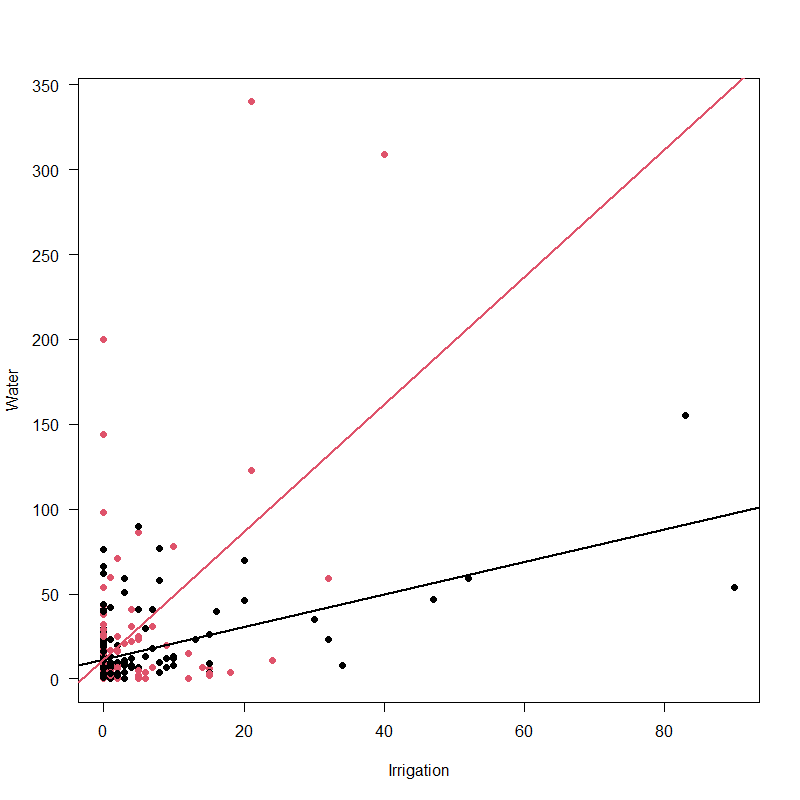
\includegraphics[width=.75\textwidth]{PS02_answers/Rplot.png}
	\end{figure}
	\vspace{6cm}
	\item [(c)] Interpret the coefficient estimate for reservation policy. \\
	\noindent In the form of y = mx + b, the coefficients give the following formula: \\
	\noindent no. of water facilities = 11.5474 + 0.9579(no. of irrigation facilities) - 0.2583(female) + 2.7978(irrigation facilities * female) \\ 
	
	\noindent This can actually be separated out into two different regression formulas for both male and female leaders, which give the following coefficients:
	\lstinputlisting[language=R, firstline=15, lastline=18]{PS02_answers/part2.R}
	\begin{verbatim}
		> reg_male$coefficients
		(Intercept)  irrigation 
		11.5474327   0.9579383 
		> reg_female$coefficients
		(Intercept)  irrigation 
		11.289121    3.755716 
	\end{verbatim}

	\noindent This displays that while the Y intercepts for the two genders are similar, the slopes are quite different, with the female regression having a much steeper slope, as shown above in Figure 2. However, as previously stated, neither have a strong R-squared statistic, with the female regression model only accounting for 25.3 \% of the variance, and with the male regression accounting for 29.5 \% of the variance in the outcome variable 

\end{enumerate}

\end{document}
